%!TEX TS-program = xelatex
\documentclass[]{friggeri-cv}
\usepackage{afterpage}
\usepackage{hyperref}
\usepackage{color}
\usepackage{xcolor}
\hypersetup{
    pdftitle={},
    pdfauthor={},
    pdfsubject={},
    pdfkeywords={},
    colorlinks=false,       % no lik border color
   allbordercolors=white    % white border color for all
}
\addbibresource{bibliography.bib}
\RequirePackage{xcolor}
\definecolor{pblue}{HTML}{0395DE}

\begin{document}
\header{Clément}{Thorey}
      {Data scientist}
      
% Fake text to add separator      
\fcolorbox{white}{gray}{\parbox{\dimexpr\textwidth-2\fboxsep-2\fboxrule}{%
.....
}}

% In the aside, each new line forces a line break
\begin{aside}
  \section{Address}
    Rue du Mont Cenis, 125
    75018, Paris, France
    ~
  \section{Tel \& Skype}
    +33 695 764 726
    thorey.clement
    ~
  \section{Mail}
    \href{mailto:clement.thorey@gmail.com}{\textbf{clement.thorey@}\\gmail.com}
    \href{mailto:thorey@ipgp.fr}{\textbf{thorey@}\\ipgp.fr}
    ~
  \section{Web \& Git}
    \href{https://github.com/cthorey}{github.com/cthorey}
    \href{http://cthorey.github.io./}{cthorey.github.io}
    \href{https://scholar.google.fr/citations?user=p5M6SxAAAAAJ&hl=fr&oi=ao}{scholar.google.fr/cthorey}
    \href{https://www.kaggle.com/cthorey/}{kaggle.com/cthorey}
    ~
  \section{Python library}
    \href{http://pdsimage.readthedocs.org/en/latest/}{pdsimage}
  ~  
  \section{Programming}
    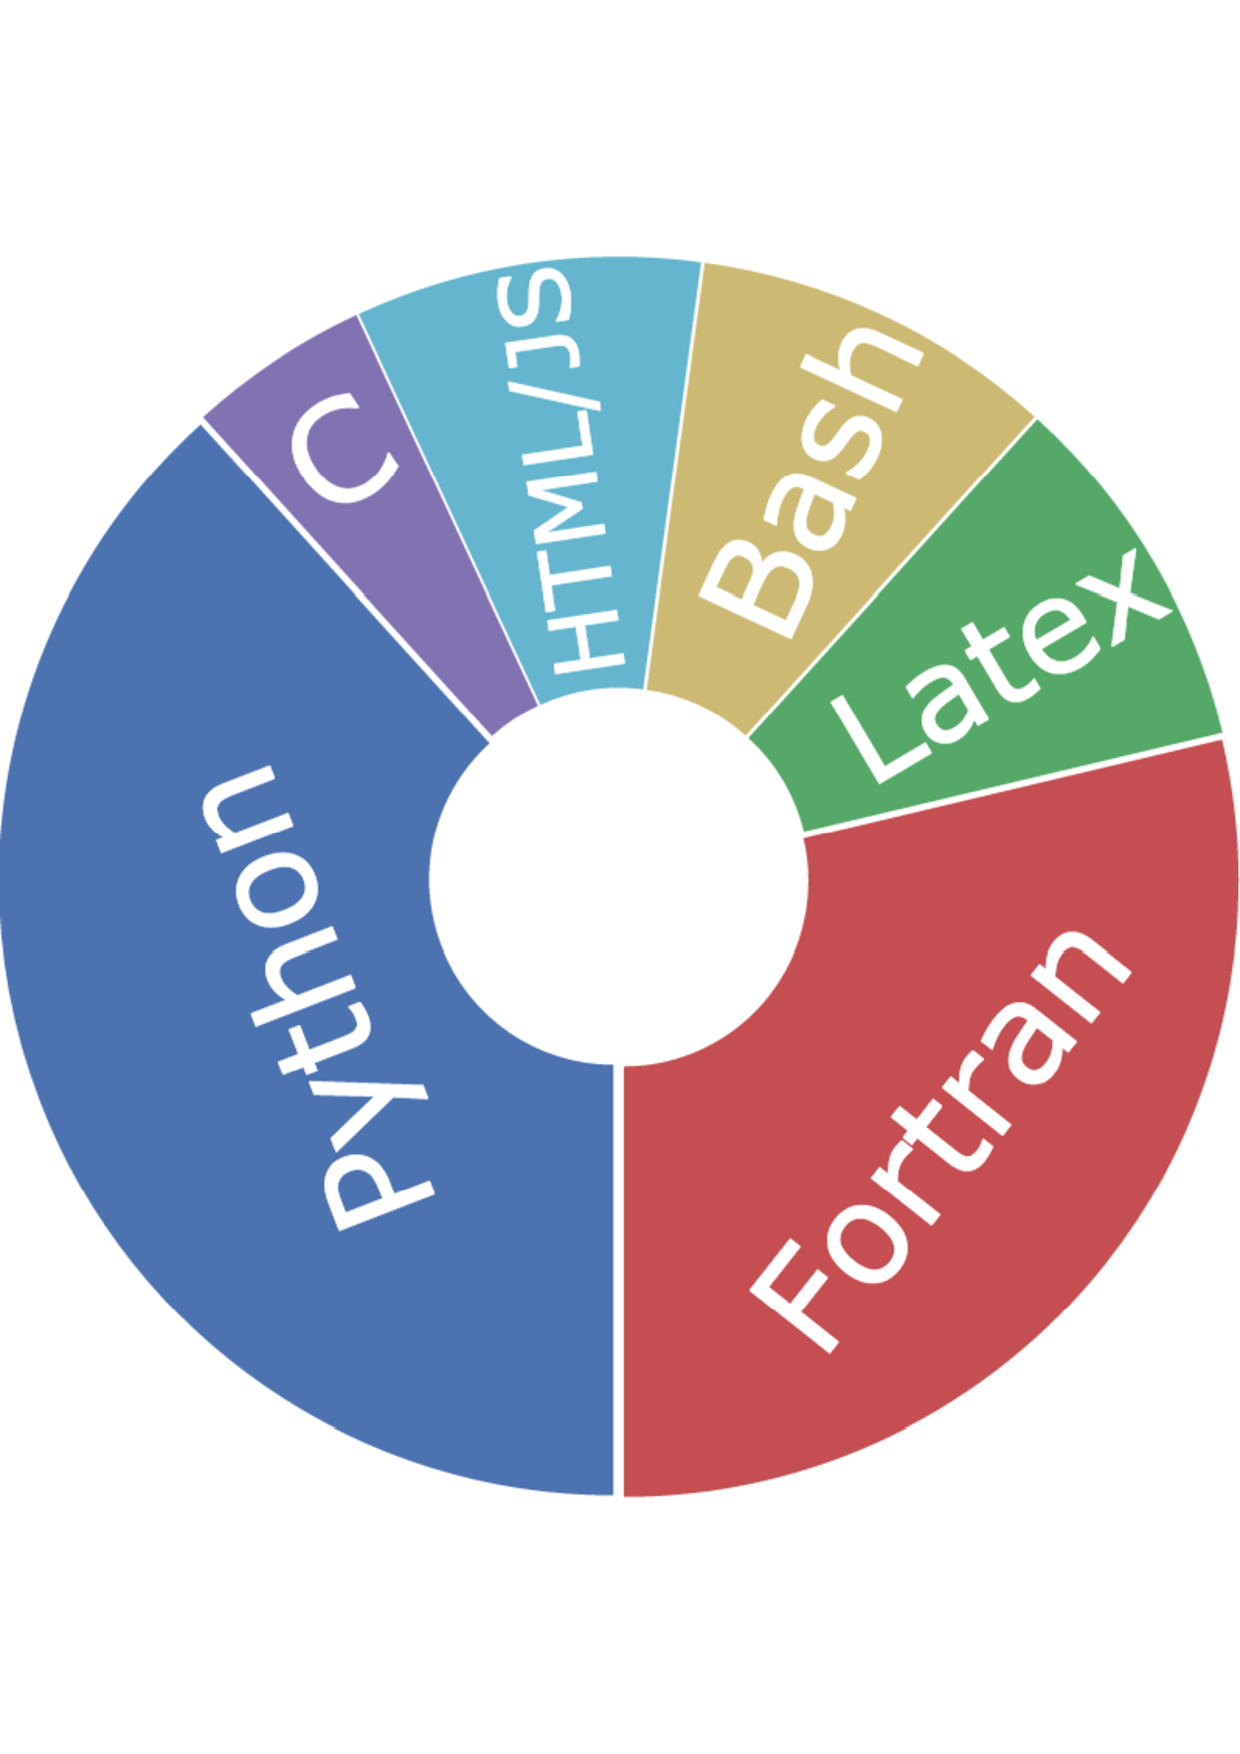
\includegraphics[scale=0.15]{img/programming.pdf}
    ~
\end{aside}

\section{Experience}
\begin{entrylist}
  \entry
    {10/12 - Now}
    {Teaching assistant}
    {Université Paris Diderot - Paris, France.}
    {Mathematics - Linear algebra, ODP, EDP, Fourrier series, Fourrier transform
    Physics - Mechanics, Experimental Physics (undergraduate level)\\
    Informatics - C (graduate level), Python (undergraduate level).\\}
  \entry
    {10/12 - 11/15}
    {PhD candidate}
    {\href{http://www.ipgp.fr/fr/pss/planetologie-sciences-spatiales}{Insitut de Physique du Globe, Paris, France.}}
    {Research interest: Intrusive magmatism on terrestrial planets. \\
    Research Method : Numerical simulation / Data analysis. \\}
   \entry
    {02/11 - 07/11}
    {Research assistant}
    {\href{http://ciiv.ucol.mx/}{Faculty of Science, University of Colima, Mexico.}}
    {Research interest: Active volcano monitoring. \\
    Research method: Seismic activity, thermal imaging, CO2 release and deformation mapping (GPS). Data preprocessing and analysis.\\}
    \entry
    {05/10 - 08/10}
    {Research assistant}
    {Benjamin Levich Institut, New York, USA.}
    {Research interest : Investigation of the periodic jamming and unjamming of dense suspensions
    in a particular geometry.\\
    Research method : Experiments, Particle tracking (PIV).\\}
\end{entrylist}

\section{Education}
\begin{entrylist}
  \entry
    {2012 - 2015}
    {PhD in Geophysics (Planetary Sciences)}
    {Institut de Physique du Globe, Paris.}
    {Thesis title: Dynamics of shallow magmatic intrusions\\
    Advisor: Chloé Michaut and Mark Wieczorek\\
    Mention: Highest distinction.}
  \entry
    {2011 - 2012}
    {Master's Degree in Earth Science}
    {Institut de Physique du Globe, Paris, France.}
    {Main subjects: Volcanology, Seismology, Geophysical Fluid Dynamics.\\
    Mention: Honors. \\}
  \entry
    {2009 - 2011}
    {Master's Degree in Theoretical Physics and Chemistry}
    {ENS Lyon, France.}
    {Courses cover the entire spectrum of physics and chemistry.\\
    Mention: Honors.\\}
  \entry
    {2008 - 2009}
    {Bachelor's Degree in in Physics and Chemistry.}
    {ENS Lyon, France.}
    {Main subjects: Physics and chemistry such as quantum physics and statistical physics.  Mathematics and computer science. \emph{Highly selective degree}.\\
    Mention: Accepted\\}
  \entry
    {2006-2008}
    {Bachelor's Degree MPSI.}
    {Université Lille 1, Lille, France.}
    {Main subjects : Mathematics, Physics and Computer Science\\
    Mention: Honors.}
\end{entrylist}

\newpage

\begin{aside}
~
~
~
  \section{Personal Skills}
    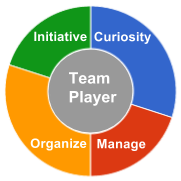
\includegraphics[scale=0.62]{img/personal.png}
    ~
  \section{Places Lived}
    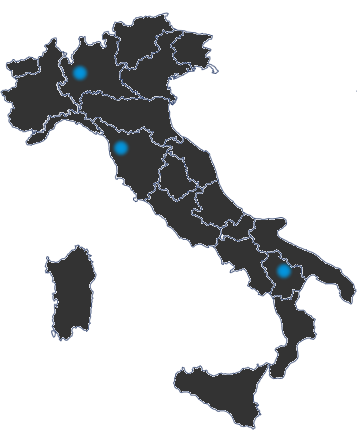
\includegraphics[scale=0.25]{img/italia.png}
    ~
  \section{Languages}
    \textbf{French}
\includegraphics[scale=0.40]{img/5stars.png}
    \textbf{English}
\includegraphics[scale=0.40]{img/4stars.png}
    \textbf{Spanish}
\includegraphics[scale=0.40]{img/4stars.png}
\end{aside}

\section{Peer-Reviewed Articles}
\begin{itemize}
\item \textbf{Thorey, C.}, Michaut,  C., 2015.  Elastic-plated gravity
  current  with  temperature-dependent  viscosity.  Journal  of  Fluid
  Mechaniscs (JFM)
\item  \textbf{Thorey,  C.},  Michaut,   C.,  Wieczorek,  M.A.,  2015.
  Gravitational  signatures of  lunar  floor-fractured craters  (FFC).
  Earth         and          Planetary         Science         Letters
  1–40. \\
  doi:10.1016/j.epsl.2015.04.021
\item \textbf{Thorey, C.}, Michaut, C., 2014. A model for the dynamics
  of crater-centered  intrusion: Application to  lunar floor-fractured
  craters.       J.       Geophys.        Res.       Planets      119,
  286–312. \\
  doi:10.1002/2013je004467
\item Michaut,  C., Baratoux, D., \textbf{Thorey,  C.}, 2013. Magmatic
  intrusions and  deglaciation at mid-latitude in  the northern plains
  of Mars. Icarus 225, 602–613. \\
  doi:10.1016/j.icarus.2013.04.015
\end{itemize}

\section{Communications in major scientific conference}
\begin{itemize}
 \item  C. Michaut and \textbf{Thorey,  C.},  Magmatism on the Moon, EGU 2016,
 Talk
 \item  \textbf{Thorey,  C.},  Floor-Fractured Craters through Machine Learning Methods, AGU Fall meeting 2015,
 Poster
 \item  \textbf{Thorey,  C.} and C. Michaut,  A General Model for Shallow Magmatic Intrus, AGU Fall meeting 2015, Poster
\item  \textbf{Thorey,  C.},  Detection of lunar floor-fractured craters using machine learning methods,EPSC 2015,
 Poster
\item  C. Michaut and \textbf{Thorey,  C.},  Magmatic intrusions in the lunar crust
 ,EPSC 2015,
 Talk
\item \textbf{Thorey,  C.} and  C. Michaut,  Effect of  a temperature-dependent
  viscosity on  the spreading  of laccoliths,  AGU Fall  meeting 2014,
  Poster
\item \textbf{Thorey,  C.}, C.  Michaut, M.  Wieczorek, Gravitational signatures
  of lunar floor  fractured craters, GRAIL science  meeting, may 2014,
  Boulder, Colorado, USA, Talk
\item \textbf{Thorey,  C.}, C.  Michaut, M.  Wieczorek, Gravitational signatures
  of lunar floor  fractured craters, LPI, Contribution  No. 2225, 45th
  LPSC, held March 2014 in The Woodlands, TX, USA, Poster
\item  \textbf{Thorey,  C.}   and Michaut  C.,  Thermal evolution  of a  magmatic
  intrusion, AGU Fall meeting 2013, Poster
\item \textbf{Thorey,  C.} and Michaut C.,  Floor-fractured craters on the Moon :
  an evidence  of past intrusive  magmatism, 44th Lunar  and Planetary
  Science Conference, held  March, 2013 in The  Woodlands, Texas.  LPI
  Contribution No. 1508, 2013, Talk.
\item \textbf{Thorey,  C.} and Michaut C.,  Floor-fractured craters on the Moon :
  an evidence  of past intrusive  magmatic activity, AGU  Fall meeting
  2012, Poster.
\item \textbf{Thorey,  C.}, November 2014, Gravitational signatures of lunar floor
  fractured  craters, Workshop  Structure and  Dynamics of  Earth-like
  Planets, Collège de France, Poster
\item  \textbf{Thorey,  C.}, November  2014, Gravitational  signatures of  lunar
  floor fractured craters, Colloque PNP, Poster
\item \textbf{Thorey,  C.}, February 2014,  Les cratères au sol fracturé: Témoins
  d'un magmatisme intrusif passé sur la Lune.  UnivEarths, Talk
\item  \textbf{Thorey,  C.},  March  2012, Formation  of  lunar  floor-fractured
  craters, Univ. de Toulouse , Poster.
\end{itemize}

\newpage

\section{Other Info}
For the Italian job market:\\
\emph{Si autorizza il trattamento delle informazioni contenute nel curriculum in conformità alle disposizioni previste dal d.lgs. 196/2003. Si dichiara altresì di essere consapevole che, in caso di dichiarazioni non veritiere, si è passibili di sanzioni penali ai sensi del DPR 445/00 oltre alla revoca dei benefici eventualmente percepiti.}
\\
\begin{flushleft}
\emph{January 14th, 2014}
\end{flushleft}
\begin{flushright}
\emph{Carmine Benedetto}
\end{flushright}


\end{document}

%%% Local Variables:
%%% mode: latex
%%% TeX-master: t
%%% End:
